\documentclass[]{article}
\usepackage{lmodern}
\usepackage{amssymb,amsmath}
\usepackage{ifxetex,ifluatex}
\usepackage{fixltx2e} % provides \textsubscript
\ifnum 0\ifxetex 1\fi\ifluatex 1\fi=0 % if pdftex
  \usepackage[T1]{fontenc}
  \usepackage[utf8]{inputenc}
\else % if luatex or xelatex
  \ifxetex
    \usepackage{mathspec}
  \else
    \usepackage{fontspec}
  \fi
  \defaultfontfeatures{Ligatures=TeX,Scale=MatchLowercase}
\fi
% use upquote if available, for straight quotes in verbatim environments
\IfFileExists{upquote.sty}{\usepackage{upquote}}{}
% use microtype if available
\IfFileExists{microtype.sty}{%
\usepackage{microtype}
\UseMicrotypeSet[protrusion]{basicmath} % disable protrusion for tt fonts
}{}
\usepackage[margin=1in]{geometry}
\usepackage{hyperref}
\hypersetup{unicode=true,
            pdftitle={SWD Behaviroial Response to Microbes when inoculated into Bluberry Juice},
            pdfauthor={Brown, JT},
            pdfborder={0 0 0},
            breaklinks=true}
\urlstyle{same}  % don't use monospace font for urls
\usepackage{color}
\usepackage{fancyvrb}
\newcommand{\VerbBar}{|}
\newcommand{\VERB}{\Verb[commandchars=\\\{\}]}
\DefineVerbatimEnvironment{Highlighting}{Verbatim}{commandchars=\\\{\}}
% Add ',fontsize=\small' for more characters per line
\usepackage{framed}
\definecolor{shadecolor}{RGB}{248,248,248}
\newenvironment{Shaded}{\begin{snugshade}}{\end{snugshade}}
\newcommand{\KeywordTok}[1]{\textcolor[rgb]{0.13,0.29,0.53}{\textbf{#1}}}
\newcommand{\DataTypeTok}[1]{\textcolor[rgb]{0.13,0.29,0.53}{#1}}
\newcommand{\DecValTok}[1]{\textcolor[rgb]{0.00,0.00,0.81}{#1}}
\newcommand{\BaseNTok}[1]{\textcolor[rgb]{0.00,0.00,0.81}{#1}}
\newcommand{\FloatTok}[1]{\textcolor[rgb]{0.00,0.00,0.81}{#1}}
\newcommand{\ConstantTok}[1]{\textcolor[rgb]{0.00,0.00,0.00}{#1}}
\newcommand{\CharTok}[1]{\textcolor[rgb]{0.31,0.60,0.02}{#1}}
\newcommand{\SpecialCharTok}[1]{\textcolor[rgb]{0.00,0.00,0.00}{#1}}
\newcommand{\StringTok}[1]{\textcolor[rgb]{0.31,0.60,0.02}{#1}}
\newcommand{\VerbatimStringTok}[1]{\textcolor[rgb]{0.31,0.60,0.02}{#1}}
\newcommand{\SpecialStringTok}[1]{\textcolor[rgb]{0.31,0.60,0.02}{#1}}
\newcommand{\ImportTok}[1]{#1}
\newcommand{\CommentTok}[1]{\textcolor[rgb]{0.56,0.35,0.01}{\textit{#1}}}
\newcommand{\DocumentationTok}[1]{\textcolor[rgb]{0.56,0.35,0.01}{\textbf{\textit{#1}}}}
\newcommand{\AnnotationTok}[1]{\textcolor[rgb]{0.56,0.35,0.01}{\textbf{\textit{#1}}}}
\newcommand{\CommentVarTok}[1]{\textcolor[rgb]{0.56,0.35,0.01}{\textbf{\textit{#1}}}}
\newcommand{\OtherTok}[1]{\textcolor[rgb]{0.56,0.35,0.01}{#1}}
\newcommand{\FunctionTok}[1]{\textcolor[rgb]{0.00,0.00,0.00}{#1}}
\newcommand{\VariableTok}[1]{\textcolor[rgb]{0.00,0.00,0.00}{#1}}
\newcommand{\ControlFlowTok}[1]{\textcolor[rgb]{0.13,0.29,0.53}{\textbf{#1}}}
\newcommand{\OperatorTok}[1]{\textcolor[rgb]{0.81,0.36,0.00}{\textbf{#1}}}
\newcommand{\BuiltInTok}[1]{#1}
\newcommand{\ExtensionTok}[1]{#1}
\newcommand{\PreprocessorTok}[1]{\textcolor[rgb]{0.56,0.35,0.01}{\textit{#1}}}
\newcommand{\AttributeTok}[1]{\textcolor[rgb]{0.77,0.63,0.00}{#1}}
\newcommand{\RegionMarkerTok}[1]{#1}
\newcommand{\InformationTok}[1]{\textcolor[rgb]{0.56,0.35,0.01}{\textbf{\textit{#1}}}}
\newcommand{\WarningTok}[1]{\textcolor[rgb]{0.56,0.35,0.01}{\textbf{\textit{#1}}}}
\newcommand{\AlertTok}[1]{\textcolor[rgb]{0.94,0.16,0.16}{#1}}
\newcommand{\ErrorTok}[1]{\textcolor[rgb]{0.64,0.00,0.00}{\textbf{#1}}}
\newcommand{\NormalTok}[1]{#1}
\usepackage{graphicx,grffile}
\makeatletter
\def\maxwidth{\ifdim\Gin@nat@width>\linewidth\linewidth\else\Gin@nat@width\fi}
\def\maxheight{\ifdim\Gin@nat@height>\textheight\textheight\else\Gin@nat@height\fi}
\makeatother
% Scale images if necessary, so that they will not overflow the page
% margins by default, and it is still possible to overwrite the defaults
% using explicit options in \includegraphics[width, height, ...]{}
\setkeys{Gin}{width=\maxwidth,height=\maxheight,keepaspectratio}
\IfFileExists{parskip.sty}{%
\usepackage{parskip}
}{% else
\setlength{\parindent}{0pt}
\setlength{\parskip}{6pt plus 2pt minus 1pt}
}
\setlength{\emergencystretch}{3em}  % prevent overfull lines
\providecommand{\tightlist}{%
  \setlength{\itemsep}{0pt}\setlength{\parskip}{0pt}}
\setcounter{secnumdepth}{0}
% Redefines (sub)paragraphs to behave more like sections
\ifx\paragraph\undefined\else
\let\oldparagraph\paragraph
\renewcommand{\paragraph}[1]{\oldparagraph{#1}\mbox{}}
\fi
\ifx\subparagraph\undefined\else
\let\oldsubparagraph\subparagraph
\renewcommand{\subparagraph}[1]{\oldsubparagraph{#1}\mbox{}}
\fi

%%% Use protect on footnotes to avoid problems with footnotes in titles
\let\rmarkdownfootnote\footnote%
\def\footnote{\protect\rmarkdownfootnote}

%%% Change title format to be more compact
\usepackage{titling}

% Create subtitle command for use in maketitle
\providecommand{\subtitle}[1]{
  \posttitle{
    \begin{center}\large#1\end{center}
    }
}

\setlength{\droptitle}{-2em}

  \title{SWD Behaviroial Response to Microbes when inoculated into Bluberry Juice}
    \pretitle{\vspace{\droptitle}\centering\huge}
  \posttitle{\par}
    \author{Brown, JT}
    \preauthor{\centering\large\emph}
  \postauthor{\par}
      \predate{\centering\large\emph}
  \postdate{\par}
    \date{August 6, 2019}


\begin{document}
\maketitle

\begin{Shaded}
\begin{Highlighting}[]
\NormalTok{#################################################################################}
\NormalTok{###Subsetting data to look at the relationship between isolate and SWD behaviors}
\NormalTok{#################################################################################}
\NormalTok{data0621=data }\OperatorTok\StringTok{ }
\StringTok{  }\NormalTok{dplyr}\OperatorTok{::}\KeywordTok{select}\NormalTok{(microbe, flies_in_treat, flies_outside, flies_in_control) }\OperatorTok\StringTok{ }
\StringTok{  }\NormalTok{dplyr}\OperatorTok{::}\KeywordTok{filter}\NormalTok{(microbe}\OperatorTok{==}\StringTok{ "C0621"}\NormalTok{) }\OperatorTok\StringTok{ }
\StringTok{  }\NormalTok{tidyr}\OperatorTok{::}\KeywordTok{gather}\NormalTok{(location, observed, flies_in_treat}\OperatorTok{:}\NormalTok{flies_in_control) }

\NormalTok{data0620=data }\OperatorTok\StringTok{ }
\StringTok{  }\NormalTok{dplyr}\OperatorTok{::}\KeywordTok{select}\NormalTok{(microbe, flies_in_treat, flies_outside, flies_in_control) }\OperatorTok\StringTok{ }
\StringTok{  }\NormalTok{dplyr}\OperatorTok{::}\KeywordTok{filter}\NormalTok{(microbe}\OperatorTok{==}\StringTok{ "C0620"}\NormalTok{) }\OperatorTok\StringTok{ }
\StringTok{  }\NormalTok{tidyr}\OperatorTok{::}\KeywordTok{gather}\NormalTok{(location, observed, flies_in_treat}\OperatorTok{:}\NormalTok{flies_in_control)}

\NormalTok{data0633=data }\OperatorTok\StringTok{ }
\StringTok{  }\NormalTok{dplyr}\OperatorTok{::}\KeywordTok{select}\NormalTok{(microbe, flies_in_treat, flies_outside, flies_in_control) }\OperatorTok\StringTok{ }
\StringTok{  }\NormalTok{dplyr}\OperatorTok{::}\KeywordTok{filter}\NormalTok{(microbe}\OperatorTok{==}\StringTok{ "C0633"}\NormalTok{) }\OperatorTok\StringTok{ }
\StringTok{  }\NormalTok{tidyr}\OperatorTok{::}\KeywordTok{gather}\NormalTok{(location, observed, flies_in_treat}\OperatorTok{:}\NormalTok{flies_in_control) }

\NormalTok{data0185=data }\OperatorTok\StringTok{ }
\StringTok{  }\NormalTok{dplyr}\OperatorTok{::}\KeywordTok{select}\NormalTok{(microbe, flies_in_treat, flies_outside, flies_in_control) }\OperatorTok\StringTok{ }
\StringTok{  }\NormalTok{dplyr}\OperatorTok{::}\KeywordTok{filter}\NormalTok{(microbe}\OperatorTok{==}\StringTok{ "C0185"}\NormalTok{) }\OperatorTok\StringTok{ }
\StringTok{  }\NormalTok{tidyr}\OperatorTok{::}\KeywordTok{gather}\NormalTok{(location, observed, flies_in_treat}\OperatorTok{:}\NormalTok{flies_in_control) }

\NormalTok{data0189=data }\OperatorTok\StringTok{ }
\StringTok{  }\NormalTok{dplyr}\OperatorTok{::}\KeywordTok{select}\NormalTok{(microbe, flies_in_treat, flies_outside, flies_in_control) }\OperatorTok\StringTok{ }
\StringTok{  }\NormalTok{dplyr}\OperatorTok{::}\KeywordTok{filter}\NormalTok{(microbe}\OperatorTok{==}\StringTok{ "C0189"}\NormalTok{) }\OperatorTok\StringTok{ }
\StringTok{  }\NormalTok{tidyr}\OperatorTok{::}\KeywordTok{gather}\NormalTok{(location, observed, flies_in_treat}\OperatorTok{:}\NormalTok{flies_in_control) }

\NormalTok{data0634=data }\OperatorTok\StringTok{ }
\StringTok{  }\NormalTok{dplyr}\OperatorTok{::}\KeywordTok{select}\NormalTok{(microbe, flies_in_treat, flies_outside, flies_in_control) }\OperatorTok\StringTok{ }
\StringTok{  }\NormalTok{dplyr}\OperatorTok{::}\KeywordTok{filter}\NormalTok{(microbe}\OperatorTok{==}\StringTok{ "C0634"}\NormalTok{) }\OperatorTok\StringTok{ }
\StringTok{  }\NormalTok{tidyr}\OperatorTok{::}\KeywordTok{gather}\NormalTok{(location, observed, flies_in_treat}\OperatorTok{:}\NormalTok{flies_in_control) }


\NormalTok{###########################################}
\NormalTok{#### Visualizing all the treatment results}
\NormalTok{###########################################}
\KeywordTok{ggplot}\NormalTok{(data, }\KeywordTok{aes}\NormalTok{(}\DataTypeTok{x=}\NormalTok{microbe, }\DataTypeTok{y=}\NormalTok{flies_in_treat))}\OperatorTok{+}\KeywordTok{geom_boxplot}\NormalTok{()}\OperatorTok{+}\KeywordTok{labs}\NormalTok{(}\DataTypeTok{x =} \StringTok{"Microbe ID"}\NormalTok{, }\DataTypeTok{y=}\StringTok{"# of Flies"}\NormalTok{)}
\end{Highlighting}
\end{Shaded}

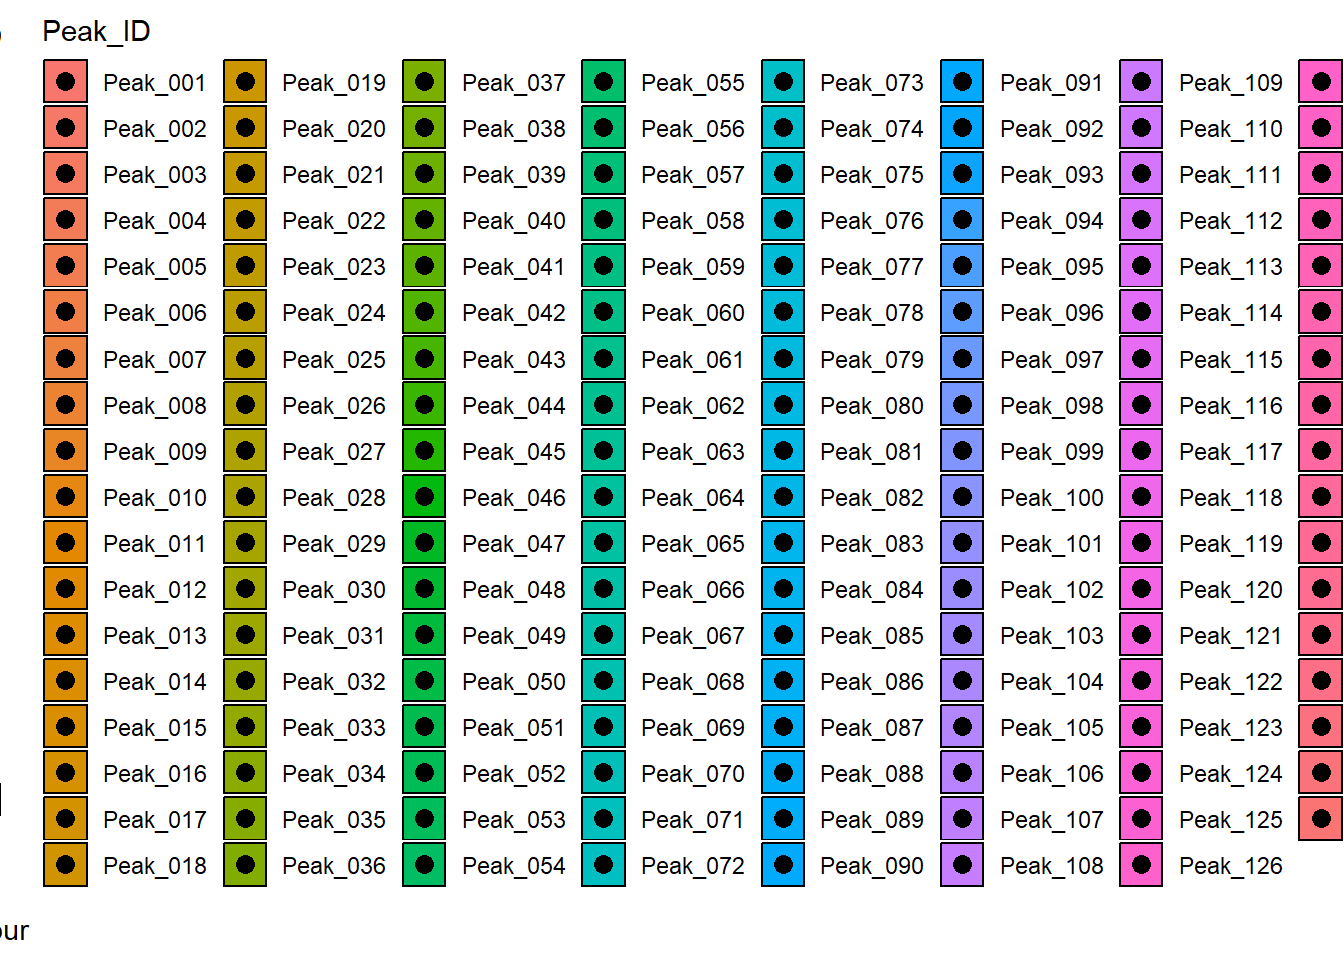
\includegraphics{SWD_MicrobeBroth_BLANKS_PRO_REP_PRELIM_DISTRIBUTIONS_files/figure-latex/unnamed-chunk-1-1.pdf}

\begin{Shaded}
\begin{Highlighting}[]
\NormalTok{data1=data }\OperatorTok\StringTok{ }
\StringTok{  }\NormalTok{dplyr}\OperatorTok{::}\KeywordTok{select}\NormalTok{(microbe, flies_in_treat, flies_outside, flies_in_control) }\OperatorTok\StringTok{ }
\StringTok{  }\NormalTok{tidyr}\OperatorTok{::}\KeywordTok{gather}\NormalTok{(location, observed, flies_in_treat}\OperatorTok{:}\NormalTok{flies_in_control)}
\KeywordTok{ggplot}\NormalTok{(data1, }\KeywordTok{aes}\NormalTok{(}\DataTypeTok{x=}\NormalTok{location, }\DataTypeTok{y=}\NormalTok{observed))}\OperatorTok{+}\KeywordTok{geom_boxplot}\NormalTok{()}\OperatorTok{+}\KeywordTok{facet_wrap}\NormalTok{(}\OperatorTok{~}\NormalTok{microbe)}\OperatorTok{+}\KeywordTok{labs}\NormalTok{(}\DataTypeTok{x =} \StringTok{"Treatment"}\NormalTok{, }\DataTypeTok{y=}\StringTok{"# of Flies"}\NormalTok{)}\OperatorTok{+}\KeywordTok{scale_x_discrete}\NormalTok{(}\DataTypeTok{labels=}\KeywordTok{c}\NormalTok{(}\StringTok{"flies_in_treat"}\NormalTok{=}\StringTok{"Treatment"}\NormalTok{, }\StringTok{"flies_in_control"}\NormalTok{=}\StringTok{"Control"}\NormalTok{, }\StringTok{"flies_outside"}\NormalTok{=}\StringTok{"No Choice"}\NormalTok{))}
\end{Highlighting}
\end{Shaded}

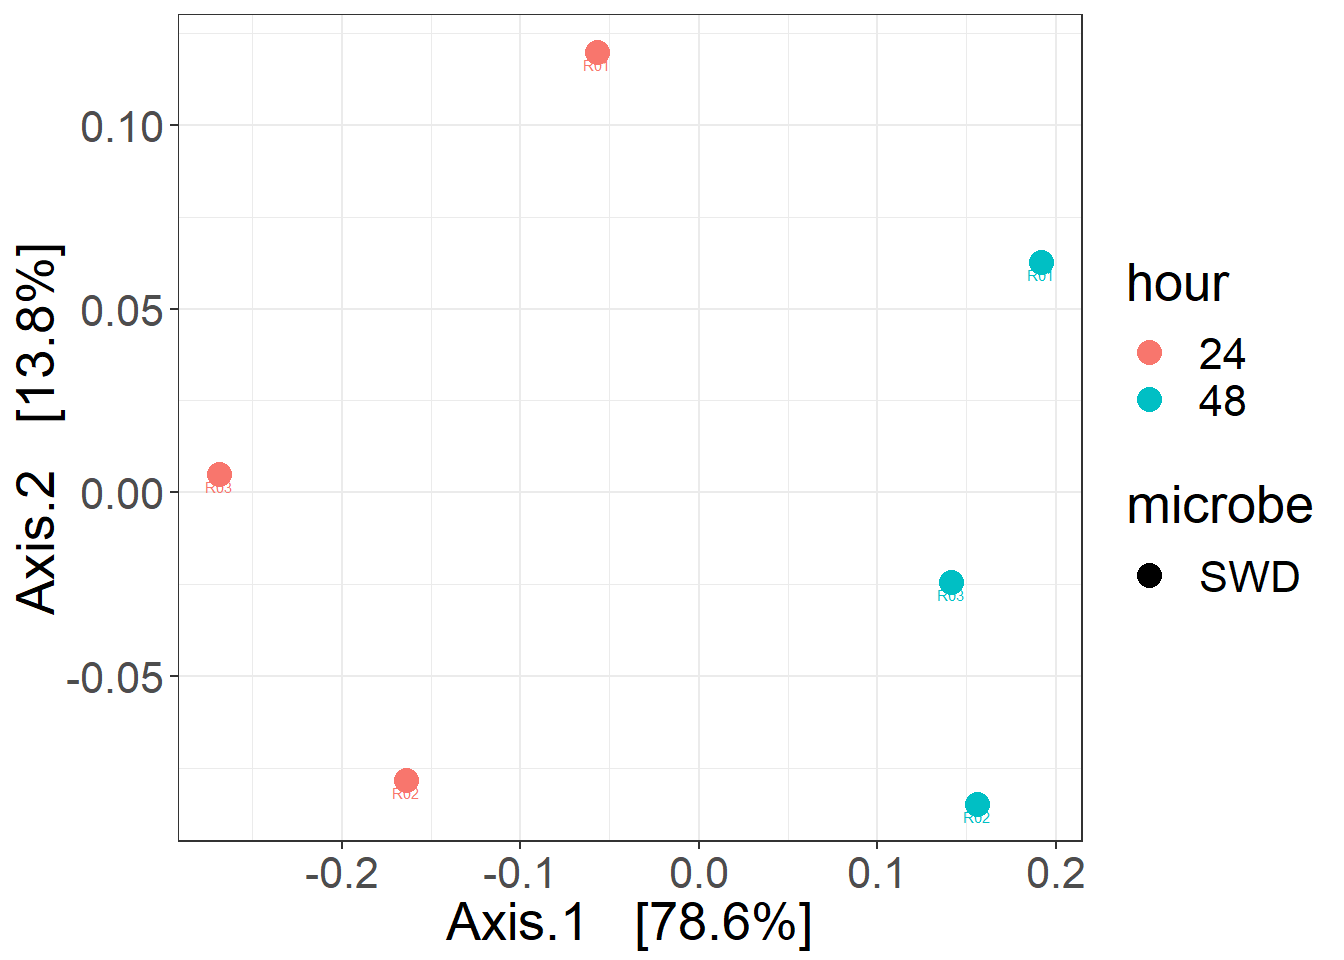
\includegraphics{SWD_MicrobeBroth_BLANKS_PRO_REP_PRELIM_DISTRIBUTIONS_files/figure-latex/unnamed-chunk-1-2.pdf}

\begin{Shaded}
\begin{Highlighting}[]
\NormalTok{##########################################################################################}
\CommentTok{#Normality Test and Linear models for the effect of each microbe on the flies in treatment}
\NormalTok{##########################################################################################}
\NormalTok{mod=}\KeywordTok{lm}\NormalTok{(flies_in_treat}\OperatorTok{~}\NormalTok{microbe,data)}
\KeywordTok{summary}\NormalTok{(mod)}
\end{Highlighting}
\end{Shaded}

\begin{verbatim}
## 
## Call:
## lm(formula = flies_in_treat ~ microbe, data = data)
## 
## Residuals:
##     Min      1Q  Median      3Q     Max 
## -9.8889 -2.8889  0.1111  3.1111  9.1111 
## 
## Coefficients:
##              Estimate Std. Error t value Pr(>|t|)    
## (Intercept)    9.8889     1.5564   6.354 7.21e-08 ***
## microbeC0189  -0.5556     2.2011  -0.252   0.8018    
## microbeC0620   1.0000     2.2011   0.454   0.6516    
## microbeC0621  -5.7778     2.2011  -2.625   0.0116 *  
## microbeC0633  -1.0000     2.2011  -0.454   0.6516    
## microbeC0634  -0.7778     2.2011  -0.353   0.7254    
## ---
## Signif. codes:  0 '***' 0.001 '**' 0.01 '*' 0.05 '.' 0.1 ' ' 1
## 
## Residual standard error: 4.669 on 48 degrees of freedom
## Multiple R-squared:  0.1933, Adjusted R-squared:  0.1093 
## F-statistic: 2.301 on 5 and 48 DF,  p-value: 0.05933
\end{verbatim}

\begin{Shaded}
\begin{Highlighting}[]
\KeywordTok{plot}\NormalTok{(mod)}
\end{Highlighting}
\end{Shaded}

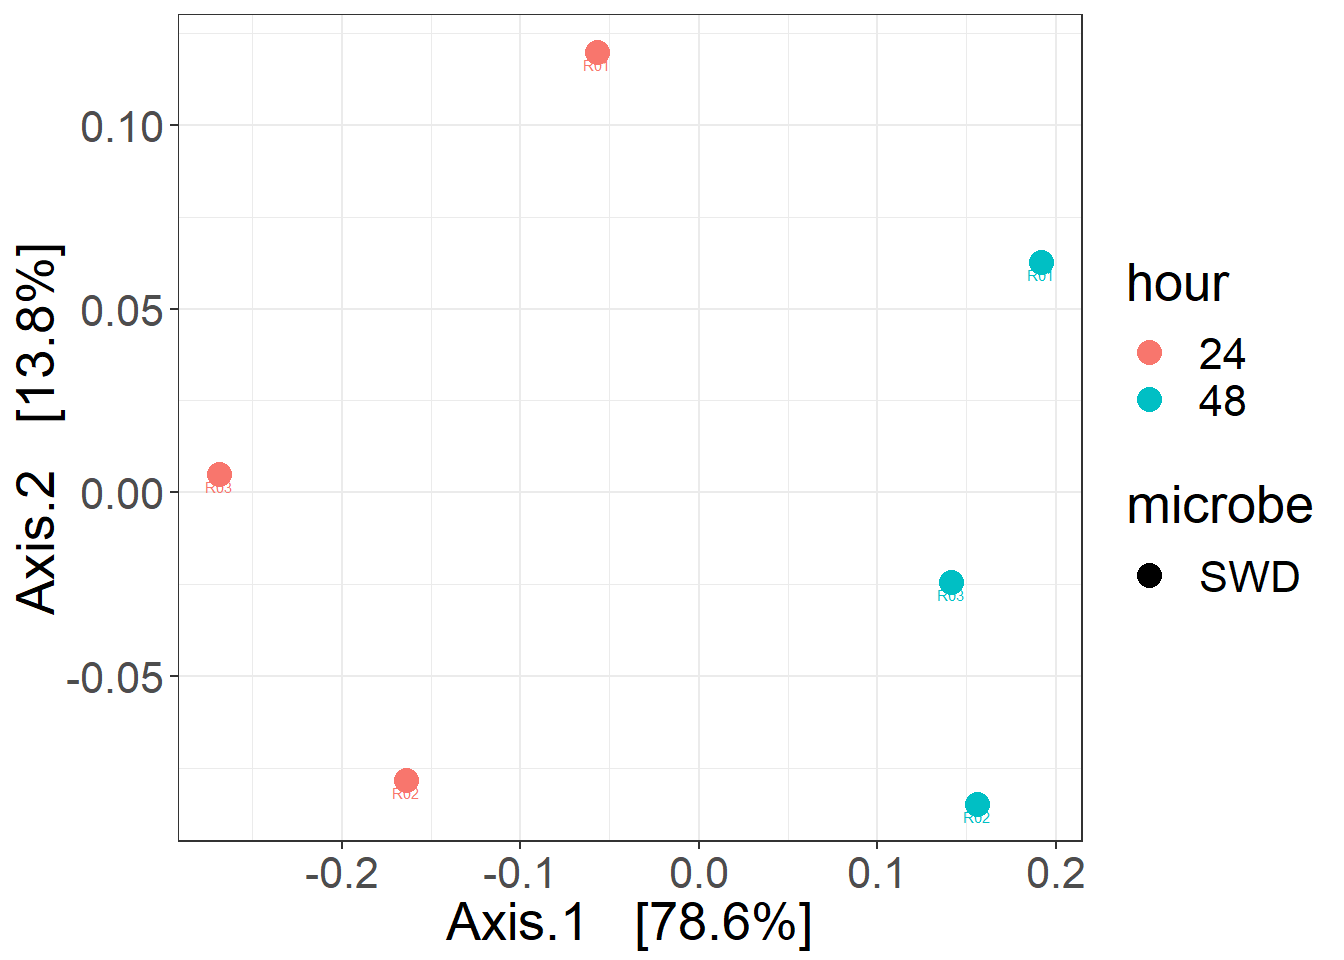
\includegraphics{SWD_MicrobeBroth_BLANKS_PRO_REP_PRELIM_DISTRIBUTIONS_files/figure-latex/unnamed-chunk-1-3.pdf}
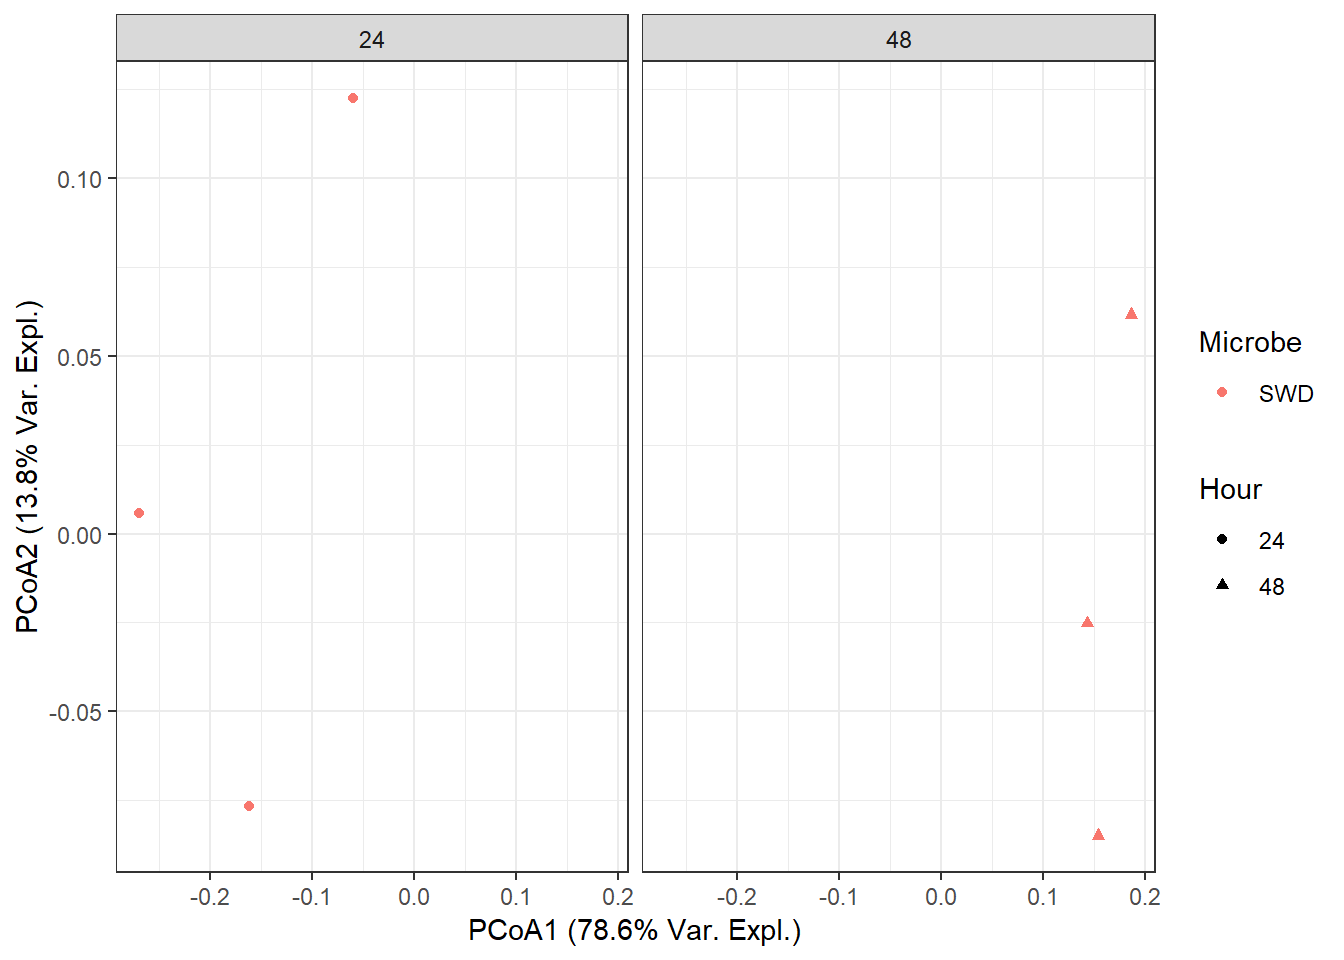
\includegraphics{SWD_MicrobeBroth_BLANKS_PRO_REP_PRELIM_DISTRIBUTIONS_files/figure-latex/unnamed-chunk-1-4.pdf}

\begin{verbatim}
## hat values (leverages) are all = 0.1111111
##  and there are no factor predictors; no plot no. 5
\end{verbatim}

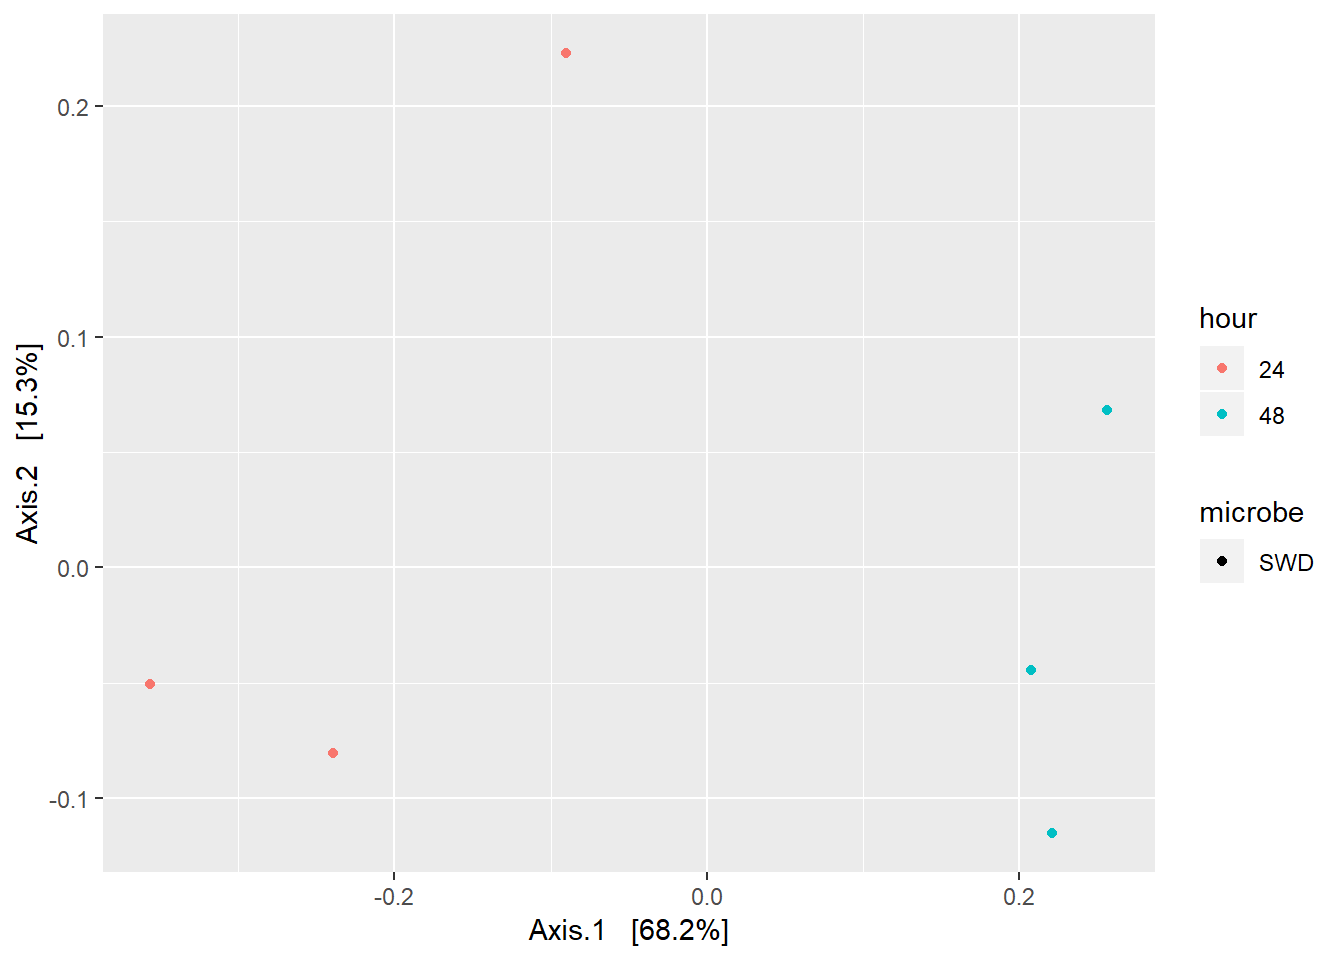
\includegraphics{SWD_MicrobeBroth_BLANKS_PRO_REP_PRELIM_DISTRIBUTIONS_files/figure-latex/unnamed-chunk-1-5.pdf}

\begin{Shaded}
\begin{Highlighting}[]
\NormalTok{mod0621=}\KeywordTok{lm}\NormalTok{(observed}\OperatorTok{~}\NormalTok{location,data0621)}
\KeywordTok{summary}\NormalTok{(mod0621)}
\end{Highlighting}
\end{Shaded}

\begin{verbatim}
## 
## Call:
## lm(formula = observed ~ location, data = data0621)
## 
## Residuals:
##     Min      1Q  Median      3Q     Max 
## -5.7778 -1.4444  0.2222  2.0556  8.2222 
## 
## Coefficients:
##                        Estimate Std. Error t value Pr(>|t|)    
## (Intercept)               8.778      1.118   7.851 4.39e-08 ***
## locationflies_in_treat   -4.667      1.581  -2.951 0.006962 ** 
## locationflies_outside    -6.000      1.581  -3.795 0.000884 ***
## ---
## Signif. codes:  0 '***' 0.001 '**' 0.01 '*' 0.05 '.' 0.1 ' ' 1
## 
## Residual standard error: 3.354 on 24 degrees of freedom
## Multiple R-squared:  0.3982, Adjusted R-squared:  0.3481 
## F-statistic: 7.941 on 2 and 24 DF,  p-value: 0.002256
\end{verbatim}

\begin{Shaded}
\begin{Highlighting}[]
\KeywordTok{plot}\NormalTok{(mod0621)}
\end{Highlighting}
\end{Shaded}

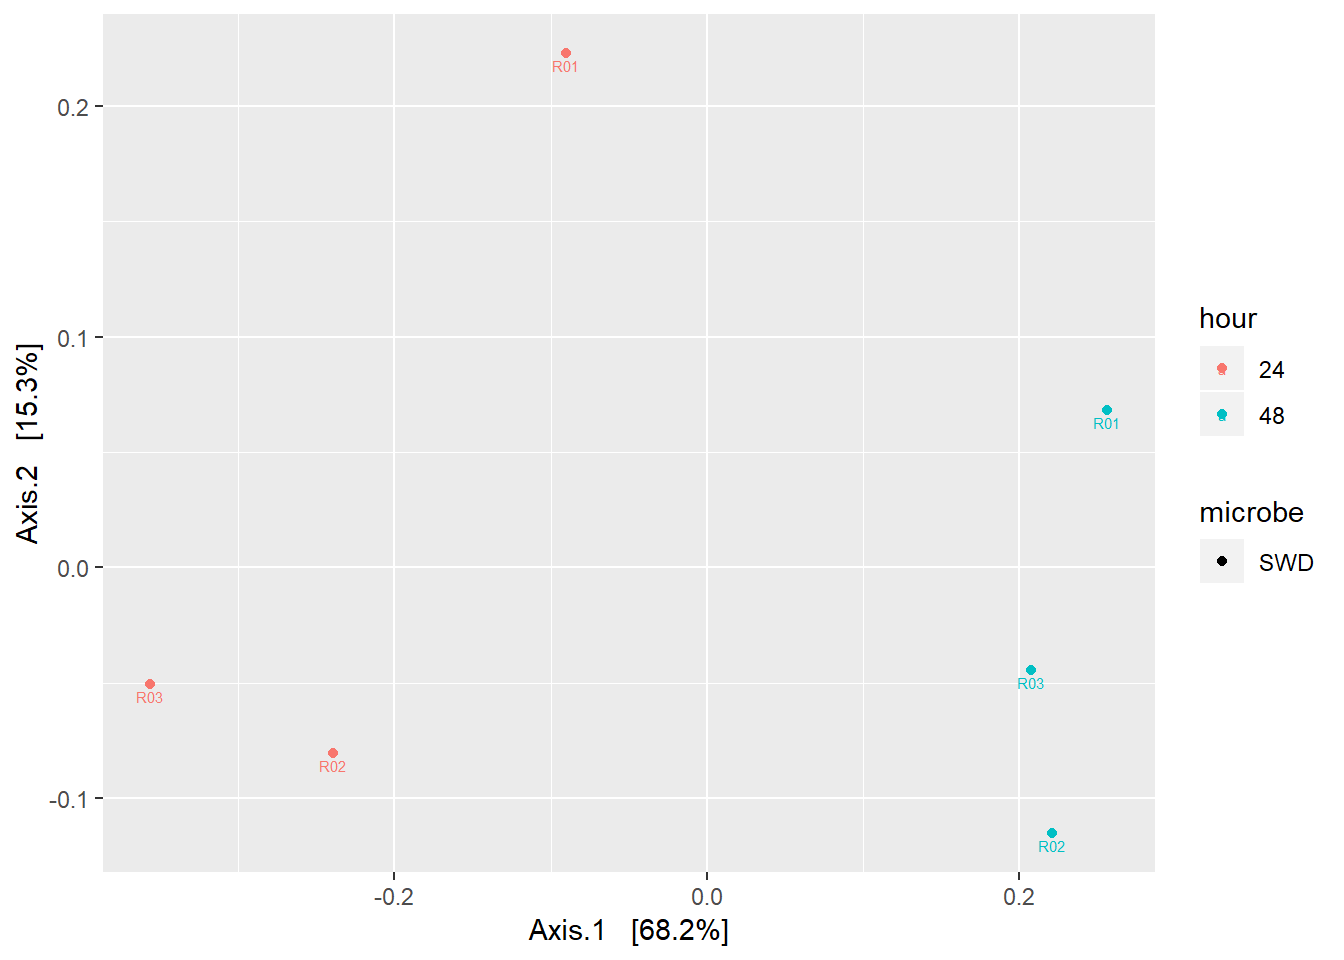
\includegraphics{SWD_MicrobeBroth_BLANKS_PRO_REP_PRELIM_DISTRIBUTIONS_files/figure-latex/unnamed-chunk-1-6.pdf}
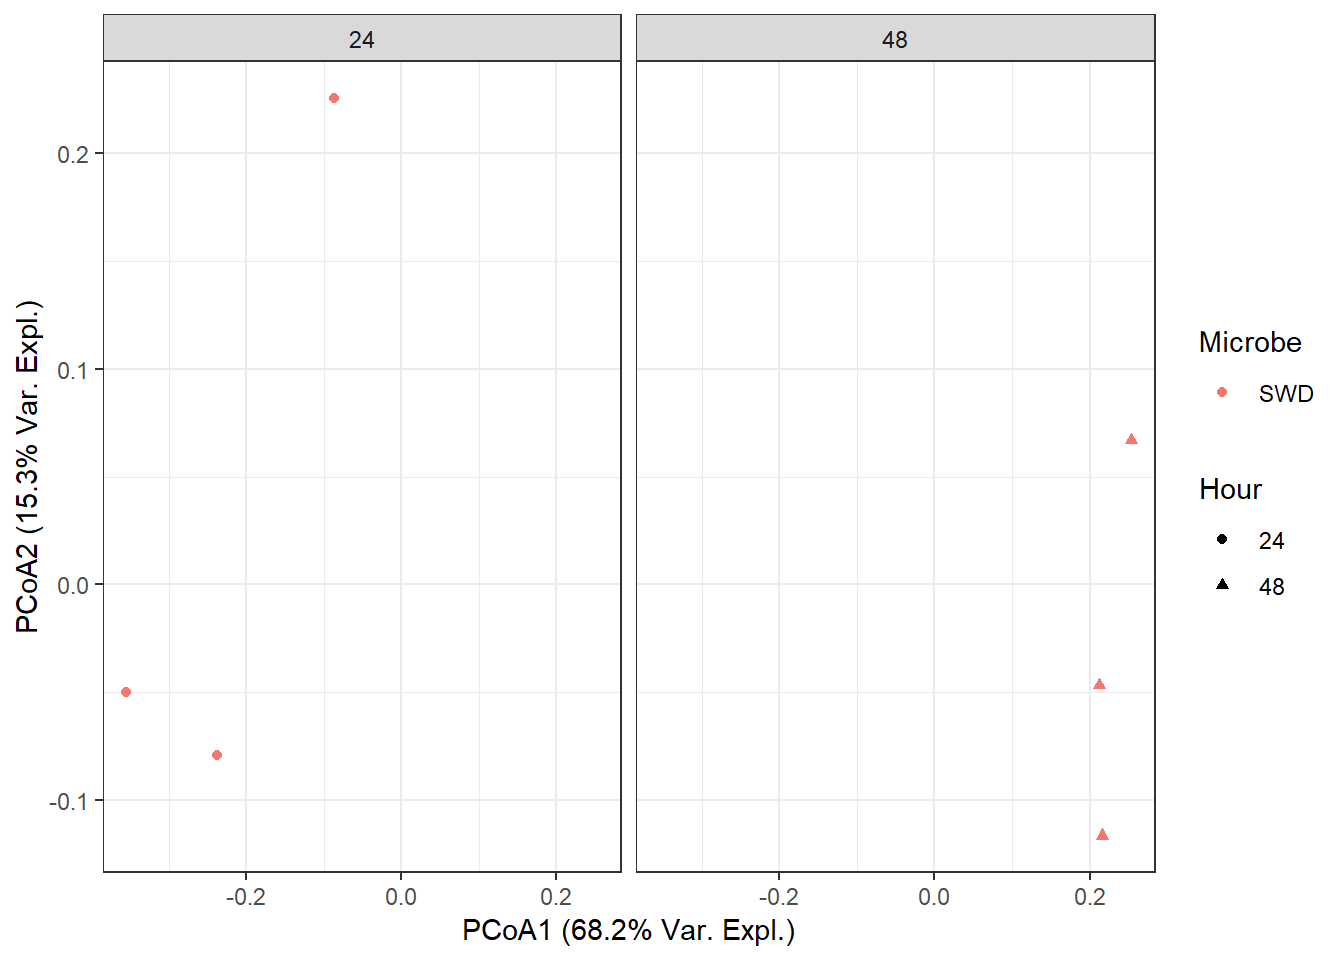
\includegraphics{SWD_MicrobeBroth_BLANKS_PRO_REP_PRELIM_DISTRIBUTIONS_files/figure-latex/unnamed-chunk-1-7.pdf}

\begin{verbatim}
## hat values (leverages) are all = 0.1111111
##  and there are no factor predictors; no plot no. 5
\end{verbatim}

\includegraphics{SWD_MicrobeBroth_BLANKS_PRO_REP_PRELIM_DISTRIBUTIONS_files/figure-latex/unnamed-chunk-1-8.pdf}

\begin{Shaded}
\begin{Highlighting}[]
\NormalTok{mod0620=}\KeywordTok{lm}\NormalTok{(observed}\OperatorTok{~}\NormalTok{location,data0620)}
\KeywordTok{summary}\NormalTok{(mod0620)}
\end{Highlighting}
\end{Shaded}

\begin{verbatim}
## 
## Call:
## lm(formula = observed ~ location, data = data0620)
## 
## Residuals:
##     Min      1Q  Median      3Q     Max 
## -6.2222 -2.2222 -0.8889  1.8333  7.7778 
## 
## Coefficients:
##                        Estimate Std. Error t value Pr(>|t|)    
## (Intercept)               6.222      1.115   5.579 9.67e-06 ***
## locationflies_in_treat    4.667      1.577   2.959  0.00684 ** 
## locationflies_outside    -3.778      1.577  -2.395  0.02477 *  
## ---
## Signif. codes:  0 '***' 0.001 '**' 0.01 '*' 0.05 '.' 0.1 ' ' 1
## 
## Residual standard error: 3.346 on 24 degrees of freedom
## Multiple R-squared:  0.5452, Adjusted R-squared:  0.5073 
## F-statistic: 14.39 on 2 and 24 DF,  p-value: 7.831e-05
\end{verbatim}

\begin{Shaded}
\begin{Highlighting}[]
\KeywordTok{plot}\NormalTok{(mod0620)}
\end{Highlighting}
\end{Shaded}

\includegraphics{SWD_MicrobeBroth_BLANKS_PRO_REP_PRELIM_DISTRIBUTIONS_files/figure-latex/unnamed-chunk-1-9.pdf}
\includegraphics{SWD_MicrobeBroth_BLANKS_PRO_REP_PRELIM_DISTRIBUTIONS_files/figure-latex/unnamed-chunk-1-10.pdf}

\begin{verbatim}
## hat values (leverages) are all = 0.1111111
##  and there are no factor predictors; no plot no. 5
\end{verbatim}

\includegraphics{SWD_MicrobeBroth_BLANKS_PRO_REP_PRELIM_DISTRIBUTIONS_files/figure-latex/unnamed-chunk-1-11.pdf}

\begin{Shaded}
\begin{Highlighting}[]
\NormalTok{mod0633=}\KeywordTok{lm}\NormalTok{(observed}\OperatorTok{~}\NormalTok{location,data0633)}
\KeywordTok{summary}\NormalTok{(mod0633)}
\end{Highlighting}
\end{Shaded}

\begin{verbatim}
## 
## Call:
## lm(formula = observed ~ location, data = data0633)
## 
## Residuals:
##     Min      1Q  Median      3Q     Max 
## -8.8889 -2.0556  0.1111  1.5556  9.1111 
## 
## Coefficients:
##                        Estimate Std. Error t value Pr(>|t|)   
## (Intercept)              4.2222     1.2222   3.455  0.00206 **
## locationflies_in_treat   4.6667     1.7285   2.700  0.01251 * 
## locationflies_outside   -0.7778     1.7285  -0.450  0.65677   
## ---
## Signif. codes:  0 '***' 0.001 '**' 0.01 '*' 0.05 '.' 0.1 ' ' 1
## 
## Residual standard error: 3.667 on 24 degrees of freedom
## Multiple R-squared:  0.326,  Adjusted R-squared:  0.2698 
## F-statistic: 5.804 on 2 and 24 DF,  p-value: 0.008787
\end{verbatim}

\begin{Shaded}
\begin{Highlighting}[]
\KeywordTok{plot}\NormalTok{(mod0633)}
\end{Highlighting}
\end{Shaded}

\includegraphics{SWD_MicrobeBroth_BLANKS_PRO_REP_PRELIM_DISTRIBUTIONS_files/figure-latex/unnamed-chunk-1-12.pdf}
\includegraphics{SWD_MicrobeBroth_BLANKS_PRO_REP_PRELIM_DISTRIBUTIONS_files/figure-latex/unnamed-chunk-1-13.pdf}

\begin{verbatim}
## hat values (leverages) are all = 0.1111111
##  and there are no factor predictors; no plot no. 5
\end{verbatim}

\includegraphics{SWD_MicrobeBroth_BLANKS_PRO_REP_PRELIM_DISTRIBUTIONS_files/figure-latex/unnamed-chunk-1-14.pdf}

\begin{Shaded}
\begin{Highlighting}[]
\NormalTok{mod0185=}\KeywordTok{lm}\NormalTok{(observed}\OperatorTok{~}\NormalTok{location,data0185)}
\KeywordTok{summary}\NormalTok{(mod0185)}
\end{Highlighting}
\end{Shaded}

\begin{verbatim}
## 
## Call:
## lm(formula = observed ~ location, data = data0185)
## 
## Residuals:
##    Min     1Q Median     3Q    Max 
## -9.889 -2.667  0.000  3.056  7.556 
## 
## Coefficients:
##                        Estimate Std. Error t value Pr(>|t|)    
## (Intercept)               5.444      1.429   3.810 0.000851 ***
## locationflies_in_treat    4.444      2.021   2.199 0.037744 *  
## locationflies_outside    -2.444      2.021  -1.210 0.238238    
## ---
## Signif. codes:  0 '***' 0.001 '**' 0.01 '*' 0.05 '.' 0.1 ' ' 1
## 
## Residual standard error: 4.287 on 24 degrees of freedom
## Multiple R-squared:  0.3323, Adjusted R-squared:  0.2767 
## F-statistic: 5.973 on 2 and 24 DF,  p-value: 0.007849
\end{verbatim}

\begin{Shaded}
\begin{Highlighting}[]
\KeywordTok{plot}\NormalTok{(mod0185)}
\end{Highlighting}
\end{Shaded}

\includegraphics{SWD_MicrobeBroth_BLANKS_PRO_REP_PRELIM_DISTRIBUTIONS_files/figure-latex/unnamed-chunk-1-15.pdf}
\includegraphics{SWD_MicrobeBroth_BLANKS_PRO_REP_PRELIM_DISTRIBUTIONS_files/figure-latex/unnamed-chunk-1-16.pdf}

\begin{verbatim}
## hat values (leverages) are all = 0.1111111
##  and there are no factor predictors; no plot no. 5
\end{verbatim}

\includegraphics{SWD_MicrobeBroth_BLANKS_PRO_REP_PRELIM_DISTRIBUTIONS_files/figure-latex/unnamed-chunk-1-17.pdf}

\begin{Shaded}
\begin{Highlighting}[]
\NormalTok{mod0189=}\KeywordTok{lm}\NormalTok{(observed}\OperatorTok{~}\NormalTok{location,data0189)}
\KeywordTok{summary}\NormalTok{(mod0189)}
\end{Highlighting}
\end{Shaded}

\begin{verbatim}
## 
## Call:
## lm(formula = observed ~ location, data = data0189)
## 
## Residuals:
##    Min     1Q Median     3Q    Max 
## -7.333 -1.778  0.000  1.722  5.667 
## 
## Coefficients:
##                        Estimate Std. Error t value Pr(>|t|)    
## (Intercept)               5.556      1.005   5.527  1.1e-05 ***
## locationflies_in_treat    3.778      1.421   2.658   0.0138 *  
## locationflies_outside    -3.556      1.421  -2.501   0.0196 *  
## ---
## Signif. codes:  0 '***' 0.001 '**' 0.01 '*' 0.05 '.' 0.1 ' ' 1
## 
## Residual standard error: 3.015 on 24 degrees of freedom
## Multiple R-squared:  0.5259, Adjusted R-squared:  0.4864 
## F-statistic: 13.31 on 2 and 24 DF,  p-value: 0.0001289
\end{verbatim}

\begin{Shaded}
\begin{Highlighting}[]
\KeywordTok{plot}\NormalTok{(mod0189)}
\end{Highlighting}
\end{Shaded}

\includegraphics{SWD_MicrobeBroth_BLANKS_PRO_REP_PRELIM_DISTRIBUTIONS_files/figure-latex/unnamed-chunk-1-18.pdf}
\includegraphics{SWD_MicrobeBroth_BLANKS_PRO_REP_PRELIM_DISTRIBUTIONS_files/figure-latex/unnamed-chunk-1-19.pdf}

\begin{verbatim}
## hat values (leverages) are all = 0.1111111
##  and there are no factor predictors; no plot no. 5
\end{verbatim}

\includegraphics{SWD_MicrobeBroth_BLANKS_PRO_REP_PRELIM_DISTRIBUTIONS_files/figure-latex/unnamed-chunk-1-20.pdf}

\begin{Shaded}
\begin{Highlighting}[]
\NormalTok{mod0634=}\KeywordTok{lm}\NormalTok{(observed}\OperatorTok{~}\NormalTok{location,data0634)}
\KeywordTok{summary}\NormalTok{(mod0634)}
\end{Highlighting}
\end{Shaded}

\begin{verbatim}
## 
## Call:
## lm(formula = observed ~ location, data = data0634)
## 
## Residuals:
##     Min      1Q  Median      3Q     Max 
## -9.1111 -2.2222 -0.2222  2.8333  7.8889 
## 
## Coefficients:
##                        Estimate Std. Error t value Pr(>|t|)   
## (Intercept)               4.222      1.269   3.326  0.00282 **
## locationflies_in_treat    4.889      1.795   2.724  0.01185 * 
## locationflies_outside    -2.000      1.795  -1.114  0.27624   
## ---
## Signif. codes:  0 '***' 0.001 '**' 0.01 '*' 0.05 '.' 0.1 ' ' 1
## 
## Residual standard error: 3.808 on 24 degrees of freedom
## Multiple R-squared:  0.3938, Adjusted R-squared:  0.3433 
## F-statistic: 7.796 on 2 and 24 DF,  p-value: 0.002462
\end{verbatim}

\begin{Shaded}
\begin{Highlighting}[]
\KeywordTok{plot}\NormalTok{(mod0634)}
\end{Highlighting}
\end{Shaded}

\includegraphics{SWD_MicrobeBroth_BLANKS_PRO_REP_PRELIM_DISTRIBUTIONS_files/figure-latex/unnamed-chunk-1-21.pdf}
\includegraphics{SWD_MicrobeBroth_BLANKS_PRO_REP_PRELIM_DISTRIBUTIONS_files/figure-latex/unnamed-chunk-1-22.pdf}

\begin{verbatim}
## hat values (leverages) are all = 0.1111111
##  and there are no factor predictors; no plot no. 5
\end{verbatim}

\includegraphics{SWD_MicrobeBroth_BLANKS_PRO_REP_PRELIM_DISTRIBUTIONS_files/figure-latex/unnamed-chunk-1-23.pdf}
\includegraphics{SWD_MicrobeBroth_BLANKS_PRO_REP_PRELIM_DISTRIBUTIONS_files/figure-latex/unnamed-chunk-1-24.pdf}

\begin{Shaded}
\begin{Highlighting}[]
\NormalTok{##########################################}
\CommentTok{#Index Plots with 95% confidence itervals}
\NormalTok{##########################################}
\NormalTok{data1=data }\OperatorTok\StringTok{ }
\StringTok{  }\KeywordTok{mutate}\NormalTok{(data1,}\DataTypeTok{escaped=}\NormalTok{total_flies}\OperatorTok{-}\NormalTok{(flies_in_treat}\OperatorTok{+}\NormalTok{flies_in_control}\OperatorTok{+}\NormalTok{flies_outside)) }\OperatorTok\StringTok{ }
\StringTok{  }\NormalTok{dplyr}\OperatorTok{::}\KeywordTok{select}\NormalTok{(microbe, flies_in_treat, flies_outside, flies_in_control, escaped) }\OperatorTok\StringTok{ }
\StringTok{  }\NormalTok{tidyr}\OperatorTok{::}\KeywordTok{gather}\NormalTok{(location, observed, flies_in_treat}\OperatorTok{:}\NormalTok{escaped)}
  

\CommentTok{# calculate CI}
\NormalTok{data1=}\KeywordTok{cbind}\NormalTok{(data1,}\DataTypeTok{CI=}\NormalTok{(}\KeywordTok{CI}\NormalTok{(data1}\OperatorTok{$}\NormalTok{observed,}\DataTypeTok{ci=}\FloatTok{0.95}\NormalTok{))) }\CommentTok{#CI(x=vector in question, ci=interval to be calculated)}
\end{Highlighting}
\end{Shaded}

\begin{verbatim}
## Warning in data.frame(..., check.names = FALSE): row names were found from
## a short variable and have been discarded
\end{verbatim}

\begin{Shaded}
\begin{Highlighting}[]
\CommentTok{# This creates the plot}
\KeywordTok{ggplot}\NormalTok{(}\DataTypeTok{data=}\NormalTok{data1,}\KeywordTok{aes}\NormalTok{(}\DataTypeTok{x=}\NormalTok{location,}\DataTypeTok{y=}\NormalTok{observed),}\DataTypeTok{group=}\NormalTok{microbe) }\OperatorTok{+}\StringTok{ }
\StringTok{  }\KeywordTok{ggtitle}\NormalTok{(}\StringTok{"Preference Index"}\NormalTok{)}\OperatorTok{+}
\StringTok{  }\KeywordTok{theme_classic}\NormalTok{()}\OperatorTok{+}
\StringTok{  }\KeywordTok{facet_wrap}\NormalTok{(}\OperatorTok{~}\NormalTok{microbe)}\OperatorTok{+}
\StringTok{  }\CommentTok{#theme(plot.title = element_text(hjust = 0.4),text = element_text(size=20), axis.text.y = element_text(angle=90, hjust=1,color="black"), axis.text.x = element_text(angle=0, hjust=1,color="black"))+ }
\StringTok{  }\KeywordTok{geom_boxplot}\NormalTok{(}\DataTypeTok{fill=}\StringTok{"grey"}\NormalTok{) }\OperatorTok{+}\StringTok{ }
\StringTok{  }\KeywordTok{labs}\NormalTok{(}\DataTypeTok{y=}\StringTok{"Index"}\NormalTok{,}\DataTypeTok{y=}\StringTok{"Observed"}\NormalTok{)}\OperatorTok{+}
\StringTok{  }\KeywordTok{ylim}\NormalTok{(}\OperatorTok{-}\FloatTok{1.0}\NormalTok{,}\FloatTok{1.0}\NormalTok{)}\OperatorTok{+}
\StringTok{  }\KeywordTok{stat_summary}\NormalTok{(}\DataTypeTok{fun.data =}\NormalTok{ mean_cl_boot, }\DataTypeTok{geom =} \StringTok{"errorbar"}\NormalTok{, }\DataTypeTok{colour =} \StringTok{"Red"}\NormalTok{,}\DataTypeTok{width=}\NormalTok{.}\DecValTok{1}\NormalTok{, }\DataTypeTok{show.legend=}\OtherTok{TRUE}\NormalTok{)}\OperatorTok{+}
\StringTok{  }\KeywordTok{stat_summary}\NormalTok{(}\DataTypeTok{fun.y =}\NormalTok{ mean, }\DataTypeTok{geom =} \StringTok{"point"}\NormalTok{, }\DataTypeTok{colour =} \StringTok{"Red"}\NormalTok{, }\DataTypeTok{show.legend=}\OtherTok{TRUE}\NormalTok{)}\OperatorTok{+}
\StringTok{  }\KeywordTok{coord_flip}\NormalTok{() }\CommentTok{#Flips the graph on the side}
\end{Highlighting}
\end{Shaded}

\begin{verbatim}
## Warning: Removed 157 rows containing non-finite values (stat_boxplot).
\end{verbatim}

\begin{verbatim}
## Warning: Removed 157 rows containing non-finite values (stat_summary).

## Warning: Removed 157 rows containing non-finite values (stat_summary).
\end{verbatim}

\begin{verbatim}
## Warning: Removed 7 rows containing missing values (geom_errorbar).
\end{verbatim}

\includegraphics{SWD_MicrobeBroth_BLANKS_PRO_REP_PRELIM_DISTRIBUTIONS_files/figure-latex/unnamed-chunk-2-1.pdf}

\begin{Shaded}
\begin{Highlighting}[]
  \CommentTok{#geom_point(data=Infect_means,aes(x=Infect_means[,], colour = "Mean"),shape=21, size=2) +}
  \CommentTok{#geom_linerange(data=Infect_mean_ci,aes(xmin=mean-ci,xmax=mean+ci,x=mean,color="95% CI")) +}
  \CommentTok{#scale_color_manual(name = "", values = c("red", "red")) +}
  \CommentTok{#guides(shape=guide_legend(label.position = "topleft",override.aes = list()))+}
  \CommentTok{#guides(shape = guide_legend(override.aes = list(size = 5))) +}
  \CommentTok{#scale_color_manual(labels = c(values = c('lightskyblue1', 'lightpink'),'95% CI', 'Mean')) +}
  \CommentTok{#Adds boxplot elements}
    \CommentTok{#Adds title using the variable title}
  \CommentTok{#Centers the title; Adjust the hjust to modify the location}
  \CommentTok{#geom_errorbarh(aes(xmin = lower, xmax = upper), width=0.2)}
  \CommentTok{#coord_flip()+ #Flips the graph on the side}
  \CommentTok{#annotate("text",x=1.35,y=-0.5,label="Mean")+}
  \CommentTok{#annotate("text",x=1.3,y=-0.5,label="Median")+}
  \CommentTok{#annotate("text",x=1.25,y=-0.5,label="95% CI")+}
  \CommentTok{#annotate("pointrange",x=1.35,y=-0.65,ymin = 0.1, ymax = 0.1, colour = "red", size = 0.1)+}
  \CommentTok{#annotate("pointrange",x=1.3,y=-0.65,y=-0.65,ymin = -0.4, ymax = -0.6,}
  \CommentTok{#         colour = "black", size = 0.4,width=0.05)+}
  \CommentTok{#annotate("rect", xmin = 1.3, xmax = 1.3, ymin = -0.6, ymax =-0.7,}
   \CommentTok{#        alpha = .2, colour="black",size=0.8)+}
  \CommentTok{#annotate("errorbar",x=1.25,y=-0.65,ymin = -0.63, ymax = -0.67,}
    \CommentTok{#       colour = "red", size = 0.4,width=0.05)}

\KeywordTok{rm}\NormalTok{(}\DataTypeTok{list=}\KeywordTok{ls}\NormalTok{())}
\end{Highlighting}
\end{Shaded}


\end{document}
